\documentclass{article}

\usepackage{listings}
\usepackage{ amssymb }
\usepackage{graphicx}
\graphicspath{ {./images/} }
\usepackage{lipsum}

\title{Formal Verification}
\author{Kevin Joshua Vinther}
\date{\today}

\begin{document}

\maketitle


%%%%%%%%%%%
% TODO: Få selve speccen af Bully Algoritmen ind, og referer til den løbende
%%%%%%%%%%%

\section{Introduction}
TODO: Confidence 1/10

Distributed Systems are very important...

A problem in Distributed Systems is the problem of leader election...

\section{Overview}
TODO: Confidence 1/10

This is the main body section.

\subsection{Terminology}
TODO: Confidence 1/10

Before explaining much of the implementation as well as how the algorithms works, it is improtant to show some of the terminology.

Failure models...
Overlay...
Logical...
Classifications...

\subsection{Leader Election}
TODO: Confidence 3/10

Leader Election is a type of algorithm in Distributed Systems, whose aim is to elect a leader from processes in a distributed systems. This is crucial for when a leader dies. The main challenge in leader election is that any process can die at any time, including the leader. Thus, if a leader dies, a new leader must be agreed upon by the other processes.
Leader election assumptions:
\begin{itemize}
        \item All nodes
        \item Fail-stop model
\end{itemize}





\subsection{Bully Algorithm}
TODO: Confidence 3/10

The Bully Algorithm is an algorithm that solves the Leader Election problem. In the bully algorithm, we assume a complete undirected graph.

\begin{lstlisting}

\end{lstlisting}

\subsection{Ring Algorithm}
TODO: Confidence 3/10

The Ring Algorithm is an algorithm that solves the Leader Election problem. In the bully algorithm, we assume a complete directed ring.


\subsection{TLA+}
TODO: Confidence 5/10

TLA+ (Temporal Language of Actions Plus) is a language for modeling specifications, and widely used for proving algorithms. It has proven to be a very useful tool for proving algorithms, because of they way the language works, by forcing you to write mathematically correct implementations, that can be tested in every possible state.

\section{Bully Algorithm}

\subsection{Setup}
TODO: Confidence 6/10: Formatting, proof-reading, ``we'', articulation, maybe some of this is not necessary? too much explanation?

The ``setup'' of the implementation consists of setting up the variables and constants we use, along with setting the initial values of the code.

\noindent\fbox{%
    \parbox{\textwidth}{%
\makebox[\textwidth]{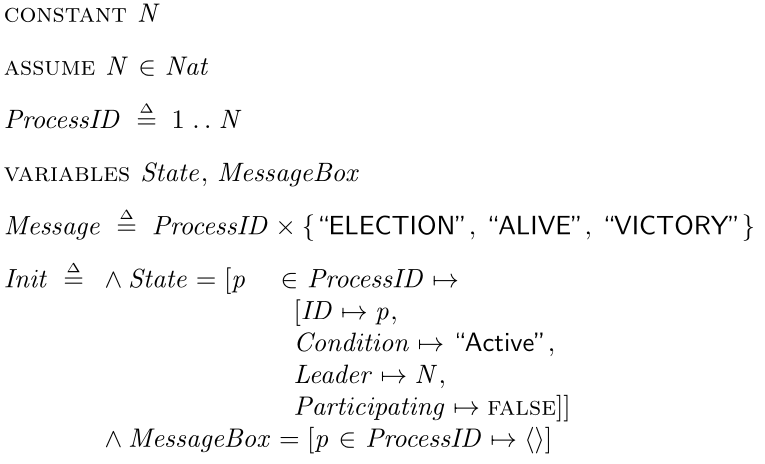
\includegraphics[scale=0.5]{setup.png}}
    }%
}


This code segment first defines a natural number constant, $N$, which chooses the number of processes in the system. The specific number $N$ is first chosen in the modeling stage, where you check the model. We then model ID's of the processes by simply making a range from 1 to and including $N$, meaning that a process can have any natural number ID up including $N$.

The variables State and MessageBox are then declared, so that we can implement their initial values in the \textit{init} function.

Before initializing, we declare that a message is the cross product between a process ID and its message ``ELECTION'', ``ALIVE'' or ``VICTORY''. This is used in the TypeOK invariant, to make sure that a message is a correct message.

In the \textit{init} function we initialize the \textit{State} and \textit{MessageBox} variables. We set State to be a tuple of processes which map to a record of the meta-information of the process. The record which each process maps to has the fields ID, Condition, Leader and Participating. The ID is set to be the process ID, $p$. We set the condition to be ``Active'', because we want each process to be active in the initial state. The ``condition'' field could be set to be ``Dead'', in which case a leader election would immediately start. We set the Leader field to be the highest process, N. We also set the \textit{Participating} field to be FALSE, as there is no election ongoing at the initial state.
We initialize the MessageBox simply by mapping each process id to an empty tuple. Thus, we end with a tuple of tuples.

With this format, we can very simply access information from any process at the current state. The condition for example, can be accessed simply by evaluating {\textit{State[$p$].Condition}}, where $p$ is the process ID. Similarly, we can access messages from a process' message box easily with \textit{(MessageBox[p])[1]} for the process ID of the sender, and \textit{(MessageBox[p])[2]} for the contents of the message.

The ease of access here makes the rest of the implementation very readable.

\subsection{Sending Messages}

TODO: Confidence 4/10: General formatting, bad formulation etc.

\noindent\fbox{%
    \parbox{\textwidth}{%
\makebox[\textwidth]{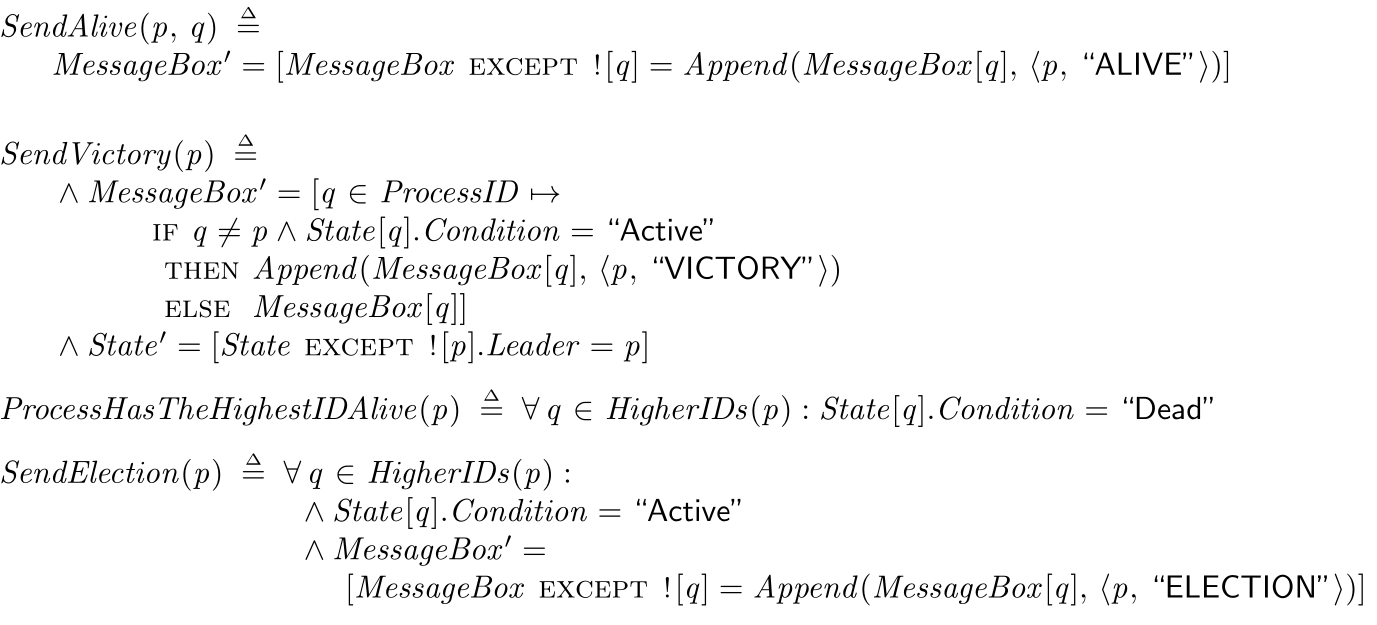
\includegraphics[scale=0.33]{sending.png}}
    }%
}

In general, with the way messages are modeled, we can send a message as simply as this:
\begin{lstlisting}
MessageBox'
    = [MessageBox EXCEPT ![q] =
       Append(MessageBox[q], <<p, ''MESSAGE'')]
\end{lstlisting}

This simply updates the MessageBox tuple for the receiving process, $q$ with a message sent from $p$ with the contents ``MESASAGE''.


\textbf{SendAlive}\\
SendAlive sends a message from process $p$ to process $q$ with the contents ``ALIVE''. The primary reason for this function is to help readability.

\textbf{SendVictory}\\
SendVictory sends a ``VICTORY'' message to every process with the condition ``Active'' which is not the process itself. The part that specifies that the receiving process should be active is not a necessity and could be left out without changing the functionality of the specification. The reason this is not done, is because it helps with a clean MessageBox. We can do this, because we assume \textbf{???? det der hvor processerne ved hvad der sker.}
Furthermore, the process $p$ which sends the message also sets its own leader to be itself, and its participation status to FALSE. Thus concluding it's own election, by assigning a new leader and not participating anymore.

\textbf{SendElection}
SendElection sends the ``ELECTION'' message to all processes with a higher id than the sender. To do this, it uses a helper function HigherIDs which is defined as such:
\begin{lstlisting}
HigherIDs(p) == {q \in ProcessID: q > p}
\end{lstlisting}

\textbf{Differences in the send functions}\\
As one may think, these functions are quite different. The SendAlive function just sends a message without doing anything else. SendVictory sends a victory to every active process that is not itself, and SendElection sends only to higher process IDs.
\textbf{TODO: Skriv hvorfor}

\subsection{Receiving Messages}
TODO: Confidence 5/10: Måske fungerer referencer til algoritme ikke helt?

\noindent\fbox{%
    \parbox{\textwidth}{%
\makebox[\textwidth]{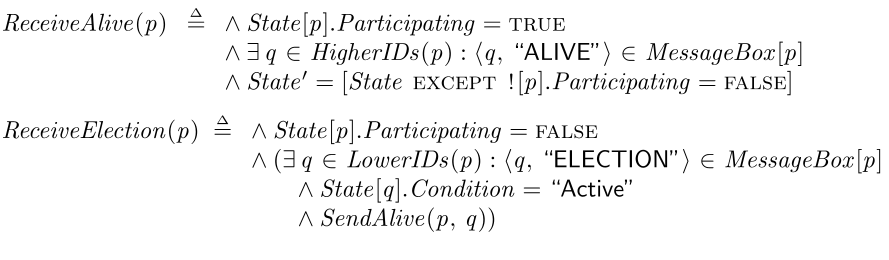
\includegraphics[scale=0.50]{receive1.png}}
\makebox[\textwidth]{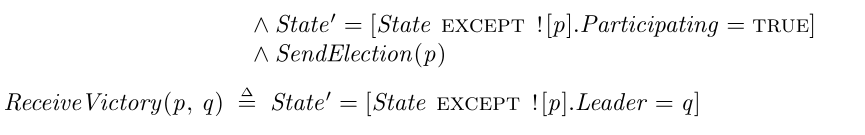
\includegraphics[scale=0.51]{receive2.png}} % scale to align
    }%
}

These functions take care of handling a message that has been received.

\textbf{ReceiveAlive}\\
\textit{If P receives an Alive from a process with a higher ID, it sends no further messages for this election and waits for a Victory message. (If there is no Victory message after a period of time, it restarts the process at the beginning.)}

This function makes sure that the process that has received the ALIVE message is currently participating in the election, and that the ALIVE message comes from a process with a higher ID. If both of these are true, the process is no longer participating in the election.

\textbf{ReceiveElection}\\
\textit{If P receives an Election message from another process with a lower ID it sends an ALIVE message back and if it has not already started an election, it starts the election process at the beginning, by sending an Election message to higher-numbered processes.}
TODO: Måske skal HigherID og LowerID bare forklares for sig selv?

This function first checks to make sure that the process is not already participating in the election. Then, it sees if the ELECTION message has come from a Lower ID, if this is the case it sends an ``ALIVE'' message to the process, if it is active. Again, making sure it is active is not a necessity, and only here to help with a clean MessageBox.
% TODO: Grunden til at de andre send funktioner er så kompliceret er fordi at receivesne bliver for clutteret
TODO: Hvorfor virker den her funktion? Burde den ikke blive FALSE hvis det ikke er fra en election?

\textbf{ReceiveVictory}\\
\textit{If P receives a Victory message, it treats the sender as the coordinator.}

ReceiveVictory changes the process' leader to be q.


\subsection{Handling Messages}
TODO: Confidence 1/10: Dårlige forklaringer, dårlig grammatik etc.

\noindent\fbox{%
    \parbox{\textwidth}{%
\makebox[\textwidth]{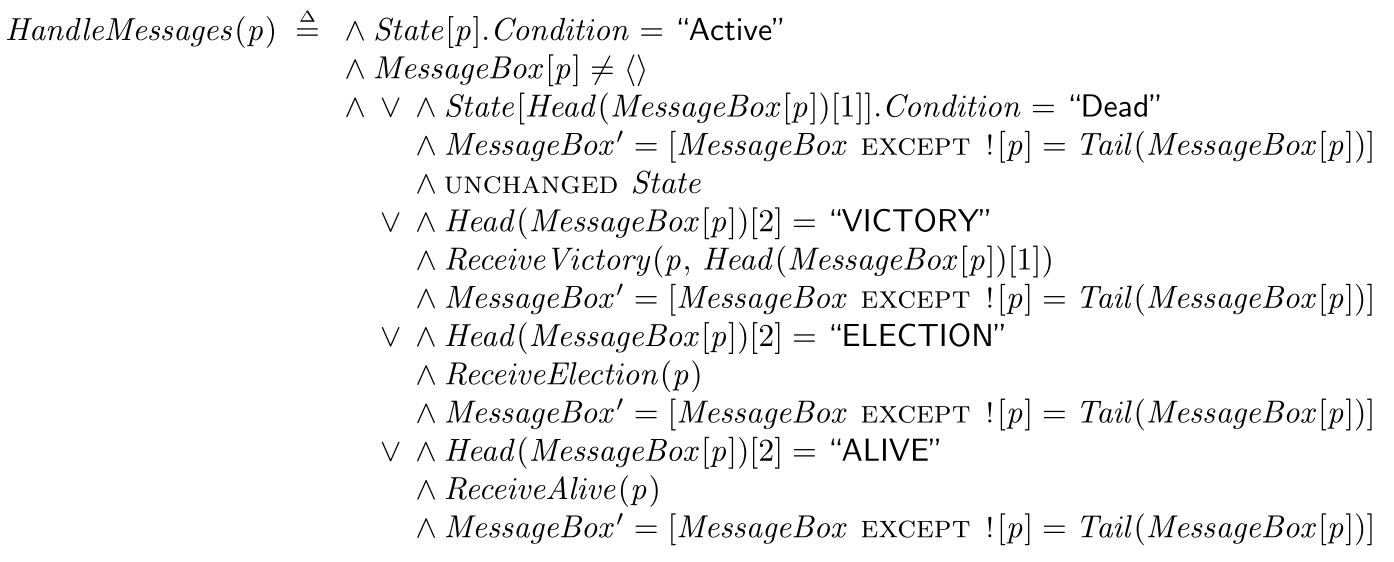
\includegraphics[scale=0.33]{handlemessages.png}} % scale to align
    }%
}

This function checks for new messages in a process' message box. It does this by looking at the first entry (the head) of the message box of process $p$. The first case is to clean up in case the process is dead. The only thing that is done, is to remove the message from the dead process. However, in the case where the process is not dead, the function looks at the contents of the message. It then calls the appropriate function depending the contents. After calling the function it removes the latest message by modifying the messagebox to be the tail.

\subsection{Checking the leader condition}
TODO: COnfidence 2/10: DÅrlig grammatik, dårlig formulering etc.\\
\noindent\fbox{%
    \parbox{\textwidth}{%
\makebox[\textwidth]{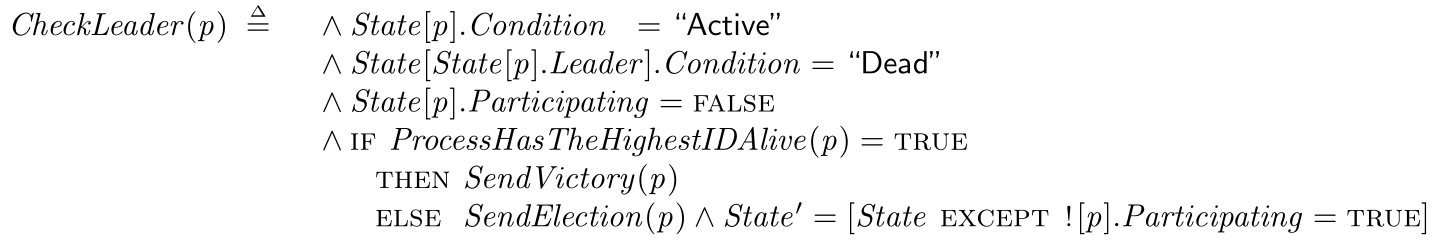
\includegraphics[scale=0.30]{checkleader.png}}
    }%
}

This function checks whether or not the current leader is dead. It only does this, if there is the process checking is not participating in an election (meaning that we assume there is no election). We then use the helper function defined up in the Sends, to see if the process has the highest ID. If this is the case, we just send a victory message, otherwise we send an election message out, and change the process to be participating in the election.
We can ``just'' say if the process has the highest ID, because we assume \textbf{hvad er det nu vi assumer siden vi bare kan sige det her? noget med at vi ved hvis processer er døde, vi ved bare ikke hvordan}
This is also the reason this function is used, rather than not getting a response and then assuming the leader process is dead.

\subsection{Next predicate and dying leader}
TODO: Confidence 2/10: For kort, dårligt beskrevet etc.

\noindent\fbox{%
    \parbox{\textwidth}{%
\makebox[\textwidth]{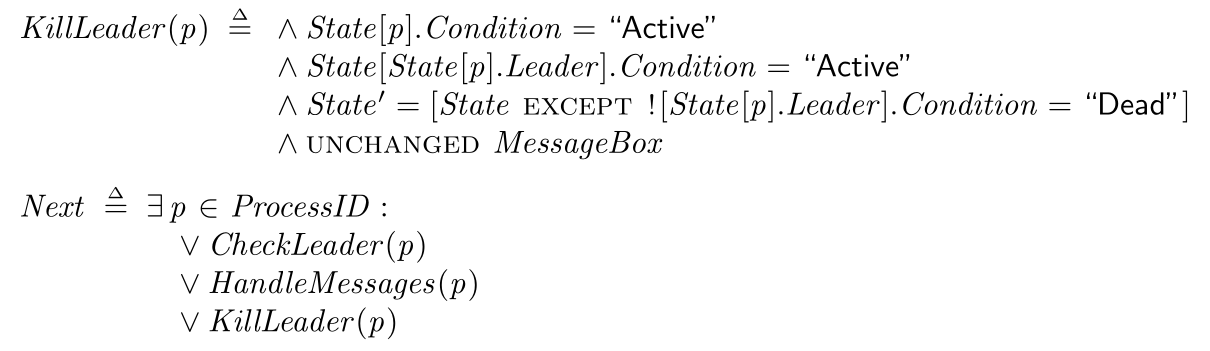
\includegraphics[scale=0.38]{killnext.png}}
    }%
}


The Next predicate is the predicate which chooses what should happen in the next state. Here we say that for some process $p$, we can either check if the leader is alive, handle any messages or kill the leader. Killing the leader is only a function to ensure the proper functioning of the spec.

\subsection{Invariants and Properties}
TODO: Confidence: 1/10, jeg har glemt at push nye variablenavne

To ensure that, while running the spec, we do not use insufficient or invalid data, we introduce invariants. One of these invariants is the TypeOK invariant, which acts as a sort of type checker for the program.

\textbf{TypeOK} \\
\begin{lstlisting}
TypeOK == \A p \in Processes :
        /\ State[p].ID \in Processes
        /\ State[p].Status \in {"Active", "Dead"}
        /\ State[p].Leader \in Processes
        /\ State[p].ElectionInProgress \in BOOLEAN
        /\ MBox \in [Processes -> Seq(Messages)]
\end{lstlisting}

TypeOK makes sure that for each process, the ID, Status, Leader, Participating and Message Box is valid. It does this by making sure that the value is part of a predefined set (such as ProcessID being the set of processes.)

\textbf{Other Invariants} \\



\section{Ring Algorithm}

\lipsum[1]

\section{Evaluation}

\lipsum[2]

\section{Conclusion}

\lipsum[3]


\end{document}
